% !TEX program = xelatex
\documentclass[UTF8,fontset=fandol]{ctexart}
\usepackage{graphicx}
\usepackage{amsmath}
\usepackage{amssymb}
\usepackage{geometry}
\usepackage{enumitem}
\geometry{a4paper, margin=2.5cm}

\title{方法章节草稿}
\author{作者}
\date{\today}



\begin{document}

\maketitle

\section{方法}

本节介绍一种面向第三方库 API 的自动化测试用例生成方法。
该方法面向的问题是：在缺少人工测试规约、API 数量较多且参数语义复杂的情况下，如何自动生成具有实际执行价值的 API 测试用例。
与传统随机测试不同，本文方法并不将输入空间视为无结构的随机取值集合，而是从 API 文档和 API 源代码中同时提取约束信息，将参数组合、参数值域、路径条件和边界条件统一到一个测试输入生成流程中。

本文方法的核心工作流程可以概括为两步：首先为每个 API 的各个参数生成多样化的测试输入候选值，然后进一步为这些输入生成对应的可执行测试用例。
具体而言，第一步依据参数边界规范为每个参数独立覆盖正常值、边界值、邻近越界值、特殊构造值等不同类型的候选输入，并将候选值区分为字面量值与代码表达式两类，以兼顾简单类型与张量、类实例等复杂对象的表示需要；第二步生成统一的 \texttt{run\_api} 调用模板，用于屏蔽普通函数、类方法、模块级 API 等不同调用形式之间的差异，再通过频次均衡采样从候选输入池中选择具体取值注入模板，形成固定预算内的完整测试用例。

\subsection{总体框架}

图~\ref{fig:method} 给出了方法的整体流程。
给定一个待测 API 集合，方法同时利用两类信息源：一类是 API 文档，其中包含函数签名、参数说明、默认值、枚举取值和部分语义约束；另一类是 API 源代码，其中包含控制流分支、参数检查逻辑和隐式路径条件。两类信息具有互补性。文档更适合描述参数的外部语义，例如某个参数是否可选、是否具有默认值、是否只能从固定集合中取值；源代码则更适合暴露真实执行逻辑，例如某个参数是否控制分支、某个取值是否触发特殊路径，以及不同参数之间是否存在文档未显式说明的交互。

整体流程可以划分为四个阶段。第一阶段是约束建模，分别从文档中抽取参数类型和参数依赖关系，从源代码中抽取路径空间和守卫条件。第二阶段是参数组合生成，先枚举候选参数组合，再根据文档约束和语义判断过滤无效组合。第三阶段是组合剪枝和边界建模，利用路径空间识别对路径选择有影响的关键参数，并在每种关键参数存在模式下保留代表性组合，同时为组合中的参数生成边界规范。第四阶段是测试输入实例化，依据边界规范生成具体参数候选值，并通过频次均衡采样组装出固定预算内的测试用例。


\begin{figure}[t]
    \centering
    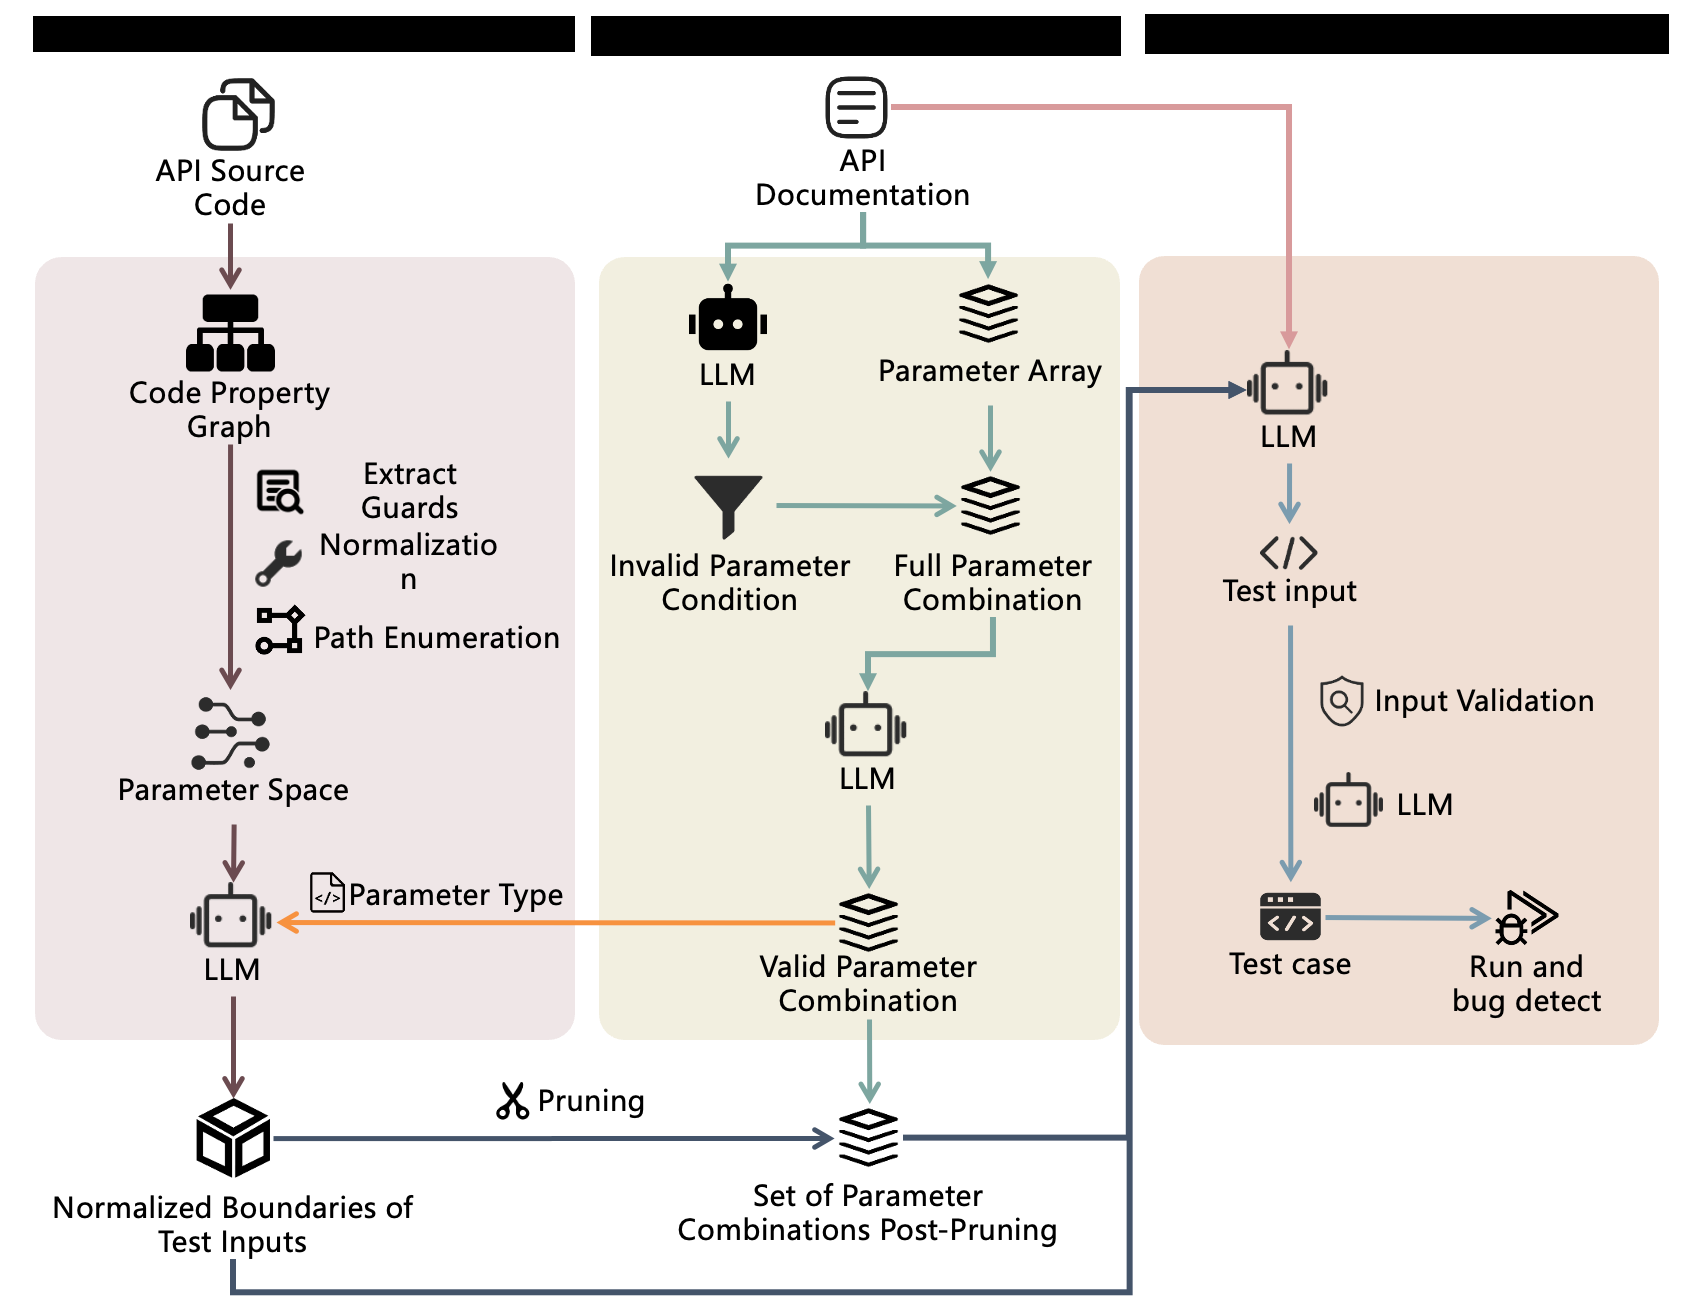
\includegraphics[width=\linewidth]{method.png}
    \caption{方法总体框架}
    \label{fig:method}
\end{figure}

形式化地，设待测 API 为 $f$，其参数集合为 $P=\{p_1,p_2,\ldots,p_n\}$。本文方法需要生成一组测试用例
\[
T_f=\{t_1,t_2,\ldots,t_k\},
\]
其中每个测试用例 $t_i$ 是参数到具体取值的部分映射，即 $t_i: P_i \rightarrow V$，$P_i \subseteq P$。这里 $P_i$ 表示一次 API 调用中显式传入的参数集合，$V$ 表示所有可能参数取值构成的值域。一个有效测试用例应满足三个要求：第一，所包含参数组合 $P_i$ 应符合文档描述的必选、互斥和共存关系；第二，参数取值应满足对应参数的类型与值域约束；第三，测试用例应尽可能覆盖由源代码路径条件诱导出的不同参数空间。

因此，本文方法不直接对完整输入空间 $P \times V$ 进行随机采样，而是将测试生成问题拆解为两个子问题：首先选择哪些参数应共同出现在同一次调用中，然后为这些参数选择哪些具体取值。前者对应参数组合生成与剪枝，后者对应边界引导的输入生成。这样的分解能够显著降低搜索空间，同时保留 API 参数语义和源代码路径语义。

\subsection{文档驱动的参数约束抽取}

API 文档通常同时包含显式签名和自然语言描述。显式签名提供参数名、参数顺序以及部分默认值；自然语言描述则提供参数用途、可选取值、类型限制以及参数之间的约束关系。由于不同第三方库的文档风格差异较大，且许多约束以自然语言而非机器可读格式出现，本文方法使用语言模型将文档中的非结构化信息转换为结构化约束。

具体而言，对于每个 API，方法将 API 名称、函数签名和文档内容组织为结构化提示，要求语言模型抽取参数级约束。抽取结果包括五类信息：
\begin{enumerate}[leftmargin=2em]
    \item 参数类型：描述每个参数的基本类型、复合类型、可选性、张量形状、枚举值或对象结构。
    \item 必选参数：调用 API 时必须显式提供的参数。
    \item 互斥参数：不能同时出现在同一次调用中的参数对或参数组。
    \item 共存参数：需要同时出现才具有语义有效性的参数集合。
    \item 条件互斥参数：仅在特定取值条件下发生冲突的参数关系。
\end{enumerate}

这一阶段的输出可以看作 API 的文档约束模型，记为
\[
D_f=(Type_f, M_f, X_f, Co_f, CX_f),
\]
其中 $Type_f$ 表示参数到类型描述的映射，$M_f$ 表示必选参数集合，$X_f$ 表示互斥参数集合，$Co_f$ 表示共存参数集合，$CX_f$ 表示条件互斥关系。该模型并不要求完全精确地表达 API 的全部语义，而是作为后续组合过滤和输入生成的基础约束。

文档约束抽取的关键意义在于，它避免了单纯依赖函数签名带来的信息缺失。许多 API 的签名只能说明参数是否有默认值，却无法说明某两个参数是否不能同时使用，或者某个字符串参数有哪些合法模式。通过语言模型提取这些隐含约束，方法能够在组合生成早期排除大量明显无效的调用形式，从而减少后续边界生成和测试执行的成本。

\subsection{源代码驱动的参数空间建模}

仅从文档中得到的参数关系通常不足以反映 API 的真实执行路径。一方面，文档可能省略内部实现中的保护条件和特殊分支；另一方面，文档往往描述的是推荐用法，而不是所有会影响执行路径的参数条件。为此，本文方法进一步分析 API 源代码，构建与参数相关的路径空间。

源代码分析首先构造代码属性图或等价的控制流表示，以捕获函数内部的条件语句、分支结构和参数检查逻辑。随后，方法抽取与 API 参数相关的守卫条件，例如类型判断、空值判断、范围判断、长度判断、枚举模式判断以及参数间关系判断。由于源代码中的条件表达式可能包含临时变量、成员访问、库内部辅助函数或语言特定语法，方法会进一步对这些条件进行规范化，使其尽可能转换为以 API 参数为中心的逻辑表达。

设源代码分析得到的路径空间为
\[
S_f=\{s_1,s_2,\ldots,s_m\},
\]
其中每个 $s_j$ 对应一组路径约束 $C_j$。方法从 $C_j$ 中识别实际影响该路径选择的参数子集 $R_j \subseteq P$。这些参数被称为路径关键参数，因为它们的出现与取值会改变 API 的内部执行行为。例如，某个参数可能控制是否进入快速路径，某个可选参数可能决定是否执行额外的类型转换，某两个参数之间的关系可能决定是否触发错误处理逻辑。

源代码驱动的参数空间建模提供了文档以外的第二类约束。与文档约束不同，路径约束不一定直接用于判定一个输入是否合法，而是用于指导测试生成关注哪些参数组合更有价值。换言之，文档约束用于减少无效输入，路径约束用于提高有效输入对程序内部行为的覆盖能力。

\subsection{参数组合构造与语义过滤}

在获得参数集合和文档约束后，方法首先生成参数集合的非空子集，得到初始组合集合
\[
\mathcal{C}_0=\{C \mid C \subseteq P, C \neq \emptyset\}.
\]
该集合表示所有可能显式传入的参数组合。直接使用 $\mathcal{C}_0$ 会产生明显的组合爆炸：当 API 包含 $n$ 个参数时，候选组合数量为 $2^n-1$。更重要的是，许多组合从 API 语义上并不成立。因此，方法首先根据文档约束对 $\mathcal{C}_0$ 进行静态过滤。若组合缺失必选参数、同时包含互斥参数，或违反共存关系，则该组合被移除。经过过滤后得到基础合法组合集合 $\mathcal{C}_1$。

静态过滤可以形式化表示为：
\[
\mathcal{C}_1=\{C \in \mathcal{C}_0 \mid M_f \subseteq C \land valid_X(C) \land valid_{Co}(C)\}.
\]
其中 $valid_X(C)$ 表示组合 $C$ 不同时包含任意互斥参数组，$valid_{Co}(C)$ 表示组合 $C$ 满足共存关系。该步骤的优点是可解释性强、成本低；不足是它只能处理已经结构化的显式规则。

然而，文档中的约束常常以自然语言形式出现，静态规则难以完整表达。例如，一些参数组合只有在特定模式下才合法，或者其合法性依赖 API 的语义背景。为解决这一问题，方法进一步使用语言模型对候选组合进行语义合法性判断。语言模型基于 API 签名、文档和当前参数组合，判断该组合是否可以构成合理调用。被判定为非法的组合被记录并从候选集合中剔除，得到语义过滤后的组合集合 $\mathcal{C}_2$。

语义过滤在整个方法中承担的是补偿角色。它并不替代静态规则，而是在静态规则之后进一步识别那些形式上未违反必选、互斥和共存关系，但根据 API 语义仍然不合理的组合。这样的两级过滤结构能够兼顾规则过滤的确定性和语言模型对自然语言语义的理解能力。

\subsection{路径感知的组合剪枝}

完整参数组合的数量随参数个数指数增长，即使经过静态和语义过滤，仍可能产生大量冗余组合。本文方法采用路径感知的组合剪枝策略，在保持路径相关覆盖能力的同时减少组合数量。

对于每个路径空间 $s_j$，方法取其关键参数集合 $R_j$，并将任意组合 $C \in \mathcal{C}_2$ 映射为一个二值存在模式：
\[
\pi_j(C)=\left(\mathbb{I}[p \in C]\right)_{p \in R_j}.
\]
该模式描述了路径相关参数在当前组合中是否出现。具有相同模式的多个组合通常会触发相似的参数存在性语义，因此不需要全部保留。对于每一种存在模式，方法仅保留两个代表性组合：参数数量最少的组合和参数数量最多的组合。前者代表最小调用上下文，后者代表更复杂的参数交互上下文。通过这种方式，方法得到剪枝后的组合集合 $\mathcal{C}_3$。

该策略可以理解为一种路径相关的等价类压缩。对于同一条路径而言，如果两个组合在路径关键参数上的存在模式完全相同，那么它们对该路径选择的贡献往往相近；二者的差异主要来自非关键参数，而这些参数不应主导组合数量。因此，方法不再保留同一存在模式下的所有组合，而是保留两个极端代表：最小组合用于测试 API 在最少显式参数下的行为，最大组合用于测试更多参数共同出现时的交互行为。

该剪枝策略的核心思想是：组合覆盖的重点不是枚举所有参数子集，而是覆盖源代码路径所关心的参数存在模式。这样既避免了组合爆炸，又保留了路径条件相关的多样性。与简单随机抽样相比，该策略具有更明确的覆盖目标；与穷举组合相比，它能够在测试预算有限的情况下显著降低生成和执行成本。

\subsection{边界规范生成}

在确定剪枝后的参数组合后，方法进一步为每个组合生成参数边界规范。边界规范的作用是将“应该测试哪些参数”进一步细化为“每个参数应该测试哪些取值区域”。该步骤综合三类信息：参数类型、路径约束和文档语义。参数类型用于确定值域形态，路径约束用于确定哪些取值能够触发特定路径，文档语义用于补充默认值、合法枚举和推荐范围。

对于数值参数，边界规范包含最小值、最大值、邻近越界值、零值、负值、极大值以及特殊浮点值。对于字符串或枚举参数，规范包含所有合法选项、非法选项、空字符串、大小写变体和包含特殊字符的字符串。对于布尔参数，规范仅包含真值和假值，以避免将整数或字符串错误地混入布尔值域。对于张量参数，规范包含形状范围、维度边界、数据类型、设备条件以及可能的稀疏或复数类型。对于复合对象，规范描述对象字段结构、字段默认值、可选字段和字段间依赖关系。

此外，源代码中的路径谓词会被转换为可执行或可检查的约束表达式。例如，分支条件、长度检查、模式选择和类型判断会被归纳为参数之间的关系约束。这些约束在后续输入生成时用于约束候选值，避免产生大量在 API 外层即被拒绝的无效输入。

边界规范生成不是简单地为每种类型填入固定模板，而是将 API 上下文纳入考虑。例如，同样是整数参数，在一个 API 中可能表示维度索引，在另一个 API 中可能表示缓存大小或模式编号。不同语义对应的有效边界不同。本文方法通过结合文档说明和路径条件，使边界值更贴近具体 API 的真实输入空间。

\subsection{边界引导的测试输入生成}

给定参数边界规范后，方法为每个参数独立生成候选测试值。候选值生成遵循两个原则。第一，类型兼容优先。生成的值必须能够到达 API 的真实执行逻辑，而不是在语言层面或简单类型检查阶段就被立即拒绝。第二，边界覆盖优先。每条边界规则至少应有一个候选值对应，以保证生成结果能够覆盖正常值、边界值和邻近越界值。

具体来说，对于数值参数，方法覆盖精确边界值、邻近越界值、零值、负值、极大值和特殊浮点值；对于枚举参数，覆盖所有合法枚举、非法枚举、空字符串、大小写变体和特殊字符；对于布尔参数，仅生成真值和假值；对于张量参数，生成不同形状、维度、数据类型和设备条件下的构造表达式；对于可选参数，额外加入空值；对于联合类型或复杂对象，分别覆盖各个可选结构。对于包含嵌套结构的复杂参数，方法优先生成完整且可直接使用的对象，而不是仅生成局部字段。

与随机生成不同，该过程要求每条边界规则至少由一个候选值覆盖，同时参考源代码中的隐式检查逻辑生成能够触发特殊路径的输入。为了保证后续执行阶段能够正确解释候选值，方法将候选值区分为字面量值和代码表达式两类。前者可直接作为参数传入，后者需要在受控命名空间中求值后再作为对象传入，例如张量构造表达式或库内部类实例。

这种候选值表示方式兼顾了通用性和可执行性。对于简单类型，直接保存字面量即可；对于张量、回调函数、配置对象或库内部类实例，仅保存序列化后的对象值往往不可行，因此使用可求值的构造表达式更适合跨阶段传递。执行阶段再根据类型标签决定是否求值，从而避免将本应作为对象传入的值误当作普通字符串。

\subsection{测试用例组装与输入校验}

在获得每个参数的候选值集合后，方法将参数组合与参数候选值结合，生成具体测试用例。对于每个 API，方法维护各参数候选值的选择频次，并采用反比权重采样策略选择候选值：
\[
w(v)=\frac{1}{count(v)+1}.
\]
其中 $count(v)$ 表示候选值 $v$ 已被选择的次数。该策略使低频候选值具有更高被选中概率，从而在有限测试预算下提高候选值覆盖均衡性。

该采样策略可以避免纯随机采样中的重复偏置。若某个候选值在前若干轮中已经多次被选中，其后续权重会下降；尚未被选中的候选值权重最高，因此更容易在后续测试中出现。这样，在固定测试预算 $k$ 下，方法能够尽量扩大候选值覆盖范围，而不是反复生成相似输入。

生成的输入在进入测试模板前需要经过输入校验。校验过程包括类型还原、代码表达式求值、参数名过滤和约束检查。对于语言模型可能生成的无效构造表达式，方法通过签名检查和语法级修复移除不被目标函数接受的关键字参数。对于不属于目标 API 签名的虚构参数，方法在执行前将其过滤。对于依赖默认值的约束，方法将显式生成的输入与默认输入合并后再进行检查，以避免因缺少上下文而错误判断约束。

测试模板用于屏蔽不同 API 调用形式之间的差异。对于普通函数，模板直接将参数传入目标函数；对于类或模块型 API，模板先完成对象实例化，再将前向输入传入对象调用过程；对于需要特殊调用约定的 API，模板保留最小必要逻辑以保证输入能够被注入执行。最终，每个通过校验的输入被注入统一的 \texttt{run\_api} 模板，形成可独立运行的测试用例。

\subsection{设计讨论}

本文方法的设计围绕三个核心问题展开。第一是如何处理参数组合爆炸。方法没有直接枚举并执行所有参数子集，而是先利用文档约束和语义判断删除无效组合，再利用路径关键参数的存在模式压缩剩余组合。这样可以在保留路径相关多样性的同时控制组合规模。第二是如何提升生成输入的有效性。方法强调类型兼容和边界覆盖，避免生成大量与 API 参数类型无关的随机值。第三是如何利用语言模型而不过度依赖语言模型。本文方法让语言模型承担自然语言理解、语义判断和复杂边界归纳等任务，同时将组合过滤、路径模式计算、候选值采样和执行前校验等步骤设计为确定性过程，以减少单次模型输出错误对整体流程的影响。

与纯文档驱动方法相比，本文方法引入源代码路径空间，因此能够识别文档未显式描述的分支条件和隐式约束。与纯静态分析方法相比，本文方法利用语言模型理解文档语义和复杂参数类型，降低了跨库适配成本。与纯随机测试方法相比，本文方法在组合层面和取值层面都具有明确覆盖目标，因此更适合在有限测试预算下生成高价值 API 测试用例。

\subsection{方法小结}

综上，本文方法通过文档理解、源代码路径分析、组合剪枝、边界规范生成、测试输入候选生成和频次均衡采样协同构造可执行 API 测试用例。整体流程可以总结为两个衔接的步骤：第一步依据边界规范为每个参数生成覆盖正常、边界、越界和特殊构造场景的多样化输入候选值，并通过字面量值与代码表达式的双轨表示兼顾简单类型与复杂对象的可执行性；第二步基于统一的 \texttt{run\_api} 调用模板，将参数组合与候选输入结合，通过反比权重的频次均衡采样在固定预算内组装出完整的可执行用例。文档提供参数语义，源代码提供路径约束，语言模型用于补足自然语言理解和复杂边界归纳能力，而路径感知剪枝和执行前输入校验则控制生成规模并提升用例质量。

\end{document}
